% Options for packages loaded elsewhere
\PassOptionsToPackage{unicode}{hyperref}
\PassOptionsToPackage{hyphens}{url}
%
\documentclass[
  ignorenonframetext,
]{beamer}
\usepackage{pgfpages}
\setbeamertemplate{caption}[numbered]
\setbeamertemplate{caption label separator}{: }
\setbeamercolor{caption name}{fg=normal text.fg}
\beamertemplatenavigationsymbolsempty
% Prevent slide breaks in the middle of a paragraph
\widowpenalties 1 10000
\raggedbottom
\setbeamertemplate{part page}{
  \centering
  \begin{beamercolorbox}[sep=16pt,center]{part title}
    \usebeamerfont{part title}\insertpart\par
  \end{beamercolorbox}
}
\setbeamertemplate{section page}{
  \centering
  \begin{beamercolorbox}[sep=12pt,center]{part title}
    \usebeamerfont{section title}\insertsection\par
  \end{beamercolorbox}
}
\setbeamertemplate{subsection page}{
  \centering
  \begin{beamercolorbox}[sep=8pt,center]{part title}
    \usebeamerfont{subsection title}\insertsubsection\par
  \end{beamercolorbox}
}
\AtBeginPart{
  \frame{\partpage}
}
\AtBeginSection{
  \ifbibliography
  \else
    \frame{\sectionpage}
  \fi
}
\AtBeginSubsection{
  \frame{\subsectionpage}
}
\usepackage{amsmath,amssymb}
\usepackage{lmodern}
\usepackage{ifxetex,ifluatex}
\ifnum 0\ifxetex 1\fi\ifluatex 1\fi=0 % if pdftex
  \usepackage[T1]{fontenc}
  \usepackage[utf8]{inputenc}
  \usepackage{textcomp} % provide euro and other symbols
\else % if luatex or xetex
  \usepackage{unicode-math}
  \defaultfontfeatures{Scale=MatchLowercase}
  \defaultfontfeatures[\rmfamily]{Ligatures=TeX,Scale=1}
  \setmainfont[BoldFont = SF Pro Rounded Semibold]{SF Pro Rounded}
  \setmathfont[]{STIX Two Math}
\fi
\usefonttheme{serif} % use mainfont rather than sansfont for slide text
% Use upquote if available, for straight quotes in verbatim environments
\IfFileExists{upquote.sty}{\usepackage{upquote}}{}
\IfFileExists{microtype.sty}{% use microtype if available
  \usepackage[]{microtype}
  \UseMicrotypeSet[protrusion]{basicmath} % disable protrusion for tt fonts
}{}
\makeatletter
\@ifundefined{KOMAClassName}{% if non-KOMA class
  \IfFileExists{parskip.sty}{%
    \usepackage{parskip}
  }{% else
    \setlength{\parindent}{0pt}
    \setlength{\parskip}{6pt plus 2pt minus 1pt}}
}{% if KOMA class
  \KOMAoptions{parskip=half}}
\makeatother
\usepackage{xcolor}
\IfFileExists{xurl.sty}{\usepackage{xurl}}{} % add URL line breaks if available
\IfFileExists{bookmark.sty}{\usepackage{bookmark}}{\usepackage{hyperref}}
\hypersetup{
  pdftitle={305 Lecture 5.1 - Subproofs},
  pdfauthor={Brian Weatherson},
  hidelinks,
  pdfcreator={LaTeX via pandoc}}
\urlstyle{same} % disable monospaced font for URLs
\newif\ifbibliography
\usepackage{graphicx}
\makeatletter
\def\maxwidth{\ifdim\Gin@nat@width>\linewidth\linewidth\else\Gin@nat@width\fi}
\def\maxheight{\ifdim\Gin@nat@height>\textheight\textheight\else\Gin@nat@height\fi}
\makeatother
% Scale images if necessary, so that they will not overflow the page
% margins by default, and it is still possible to overwrite the defaults
% using explicit options in \includegraphics[width, height, ...]{}
\setkeys{Gin}{width=\maxwidth,height=\maxheight,keepaspectratio}
% Set default figure placement to htbp
\makeatletter
\def\fps@figure{htbp}
\makeatother
\setlength{\emergencystretch}{3em} % prevent overfull lines
\providecommand{\tightlist}{%
  \setlength{\itemsep}{0pt}\setlength{\parskip}{0pt}}
\setcounter{secnumdepth}{-\maxdimen} % remove section numbering
\let\Tiny=\tiny

 \setbeamertemplate{navigation symbols}{} 

% \usetheme{Madrid}
 \usetheme[numbering=none, progressbar=foot]{metropolis}
 \usecolortheme{wolverine}
 \usepackage{color}
 \usepackage{MnSymbol}
% \usepackage{movie15}

\usepackage{amssymb}% http://ctan.org/pkg/amssymb
\usepackage{pifont}% http://ctan.org/pkg/pifont
\newcommand{\cmark}{\ding{51}}%
\newcommand{\xmark}{\ding{55}}%

\DeclareSymbolFont{symbolsC}{U}{txsyc}{m}{n}
\DeclareMathSymbol{\boxright}{\mathrel}{symbolsC}{128}
\DeclareMathAlphabet{\mathpzc}{OT1}{pzc}{m}{it}

 \usepackage{tikz-qtree}
% \usepackage{markdown}
%\RequirePackage{bussproofs}
\RequirePackage[tableaux]{prooftrees}
\usetikzlibrary{arrows.meta}
 \forestset{line numbering, close with = x}
% Allow for easy commas inside trees
\renewcommand{\,}{\text{, }}


\usepackage{tabulary}

\usepackage{open-logic-config}

\setlength{\parskip}{1ex plus 0.5ex minus 0.2ex}

\AtBeginSection[]
{
\begin{frame}
	\Huge{\color{darkblue} \insertsection}
\end{frame}
}

\renewenvironment*{quote}	
	{\list{}{\rightmargin   \leftmargin} \item } 	
	{\endlist }

\definecolor{darkgreen}{rgb}{0,0.7,0}
\definecolor{darkblue}{rgb}{0,0,0.8}

\newcommand{\starttab}{\begin{center}
\vspace{6pt}
\begin{tabular}}

\newcommand{\stoptab}{\end{tabular}
\vspace{6pt}
\end{center}
\noindent}


\newcommand{\sif}{\rightarrow}
\newcommand{\siff}{\leftrightarrow}
\newcommand{\EF}{\end{frame}}


\newcommand{\TreeStart}[1]{
%\end{frame}
\begin{frame}
\begin{center}
\begin{tikzpicture}[scale=#1]
\tikzset{every tree node/.style={align=center,anchor=north}}
%\Tree
}

\newcommand{\TreeEnd}{
\end{tikzpicture}
%\end{center}
}

\newcommand{\DisplayArg}[2]{
\begin{enumerate}
{#1}
\end{enumerate}
\vspace{-6pt}
\hrulefill

%\hspace{14pt} #2
%{\addtolength{\leftskip}{14pt} #2}
\begin{quote}
{\normalfont #2}
\end{quote}
\vspace{12pt}
}

\newenvironment{ProofTree}[1][1]{
\begin{center}
\begin{tikzpicture}[scale=#1]
\tikzset{every tree node/.style={align=center,anchor=south}}
}
{
\end{tikzpicture}
\end{center}
}

\newcommand{\TreeFrame}[2]{
\begin{columns}[c]
\column{0.5\textwidth}
\begin{center}
\begin{prooftree}{}
#1
\end{prooftree}
\end{center}
\column{0.45\textwidth}
%\begin{markdown}
#2
%\end{markdown}
\end{columns}
}

\newcommand{\ScaledTreeFrame}[3]{
\begin{columns}[c]
\column{0.5\textwidth}
\begin{center}
\scalebox{#1}{
\begin{prooftree}{}
#2
\end{prooftree}
}
\end{center}
\column{0.45\textwidth}
%\begin{markdown}
#3
%\end{markdown}
\end{columns}
}

\usepackage[bb=boondox]{mathalfa}
\DeclareMathAlphabet{\mathbx}{U}{BOONDOX-ds}{m}{n}
\SetMathAlphabet{\mathbx}{bold}{U}{BOONDOX-ds}{b}{n}
\DeclareMathAlphabet{\mathbbx} {U}{BOONDOX-ds}{b}{n}


\newenvironment{oltableau}{\center\tableau{}} %wff format={anchor = base west}}}
       {\endtableau\endcenter}
       
\newcommand{\formula}[1]{$#1$}

\usepackage{tabulary}
\usepackage{booktabs}

\def\begincols{\begin{columns}}
\def\begincol{\begin{column}}
\def\endcol{\end{column}}
\def\endcols{\end{columns}}

\usepackage[italic]{mathastext}
\usepackage{nicefrac}

\definecolor{mygreen}{RGB}{0, 100, 0}
\definecolor{mypink2}{RGB}{219, 48, 122}
\definecolor{dodgerblue}{RGB}{30,144,255}

%\def\True{\textcolor{dodgerblue}{\text{T}}}
%\def\False{\textcolor{red}{\text{F}}}

\def\True{\mathbb{T}}
\def\False{\mathbb{F}}

% This is because arguments didn't have enough space after them
\usepackage{etoolbox}
\AfterEndEnvironment{description}{\vspace{9pt}}
\AfterEndEnvironment{oltableau}{\vspace{9pt}}
\BeforeBeginEnvironment{oltableau}{\vspace{9pt}}
\AfterEndEnvironment{center}{\vspace{12pt}}
\BeforeBeginEnvironment{tabular}{\vspace{9pt}}

\setlength\heavyrulewidth{0pt}
\setlength\lightrulewidth{0pt}

%\def\toprule{}
%\def\bottomrule{}
%\def\midrule{}

\setbeamertemplate{caption}{\raggedright\insertcaption}

\ifluatex
  \usepackage{selnolig}  % disable illegal ligatures
\fi

\title{305 Lecture 5.1 - Subproofs}
\author{Brian Weatherson}
\date{}

\begin{document}
\frame{\titlepage}

\begin{frame}{Plan}
\protect\hypertarget{plan}{}
This lecture discusses how subproofs work
\end{frame}

\begin{frame}{Associated Reading}
\protect\hypertarget{associated-reading}{}
forall x, section 16.5.
\end{frame}

\begin{frame}{Example of Subproof}
\protect\hypertarget{example-of-subproof}{}
\begin{columns}[c]
\begin{column}{0.48\textwidth}
\begin{figure}
\centering
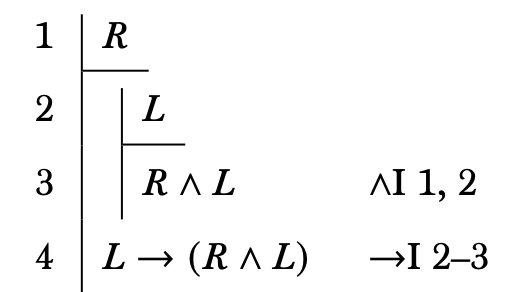
\includegraphics{4_7c.png}
\caption{A proof with a subproof}
\end{figure}
\end{column}

\begin{column}{0.48\textwidth}
\begin{itemize}
\tightlist
\item
  The subproof is the part of the proof that runs from 2 to 3.
\item
  Line 2 introduces a subproof - it is indented, and has a bar under the
  first line.
\end{itemize}
\end{column}
\end{columns}
\end{frame}

\begin{frame}{Example of Subproof}
\protect\hypertarget{example-of-subproof-1}{}
\begin{columns}[c]
\begin{column}{0.48\textwidth}
\begin{figure}
\centering
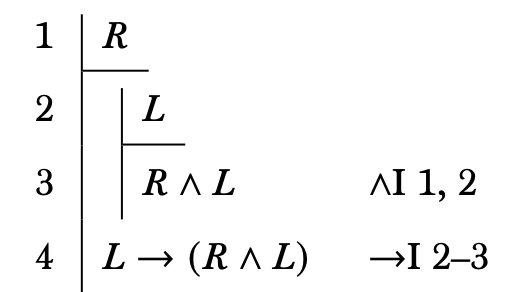
\includegraphics{4_7c.png}
\caption{A proof with a subproof}
\end{figure}
\end{column}

\begin{column}{0.48\textwidth}
Line 3 turns out not to be particularly important - subproofs just end
when they end, there isn't anything that makes it stand out as the end.
\end{column}
\end{columns}
\end{frame}

\begin{frame}{Example of Subproof}
\protect\hypertarget{example-of-subproof-2}{}
\begin{columns}[c]
\begin{column}{0.48\textwidth}
\begin{figure}
\centering
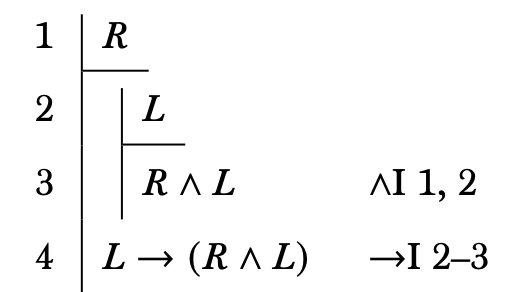
\includegraphics{4_7c.png}
\caption{A proof with a subproof}
\end{figure}
\end{column}

\begin{column}{0.48\textwidth}
\begin{itemize}
\tightlist
\item
  What is important is line 4, when we return to the main proof.
\item
  Moving back up one level like this is called \textbf{discharging} an
  assumption (125).
\end{itemize}
\end{column}
\end{columns}
\end{frame}

\begin{frame}
\begin{columns}[c]
\begin{column}{0.48\textwidth}
\begin{figure}
\centering
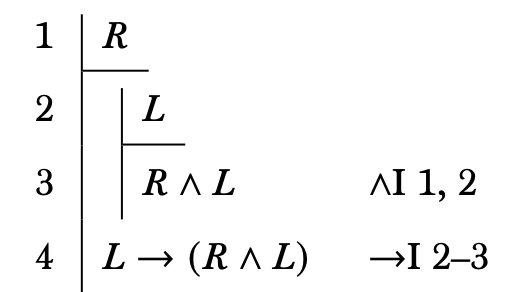
\includegraphics{4_7c.png}
\caption{A proof with a subproof}
\end{figure}
\end{column}

\begin{column}{0.48\textwidth}
When we are still in the subproof, we haven't moved back one step to the
left, everything we assert is said to follow both from the premises and
from the assumption at the start of the subproof.
\end{column}
\end{columns}
\end{frame}

\begin{frame}
\begin{columns}[c]
\begin{column}{0.48\textwidth}
\begin{figure}
\centering
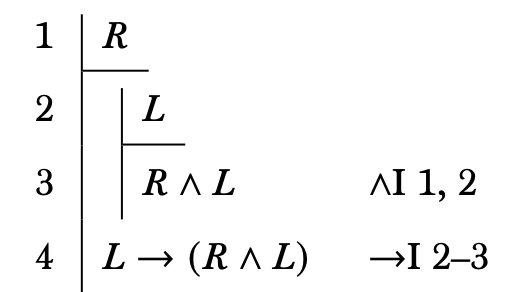
\includegraphics{4_7c.png}
\caption{A proof with a subproof}
\end{figure}
\end{column}

\begin{column}{0.48\textwidth}
\begin{itemize}
\tightlist
\item
  Once we close the subproof, we are saying that things follow just from
  the initial premises.
\item
  That's the sense in which the assumption is discharged.
\end{itemize}
\end{column}
\end{columns}
\end{frame}

\begin{frame}{Rules on Subproofs}
\protect\hypertarget{rules-on-subproofs}{}
\begin{enumerate}
\tightlist
\item
  Only some very special rules let you appeal to subproofs.
\item
  Once a subproof is closed, you can't appeal to any part of it, just to
  the existence of the subproof.
\item
  You can (typically) only close one subproof at a time.
\end{enumerate}
\end{frame}

\begin{frame}{What Could go Wrong?!}
\protect\hypertarget{what-could-go-wrong}{}
\begin{figure}
\centering
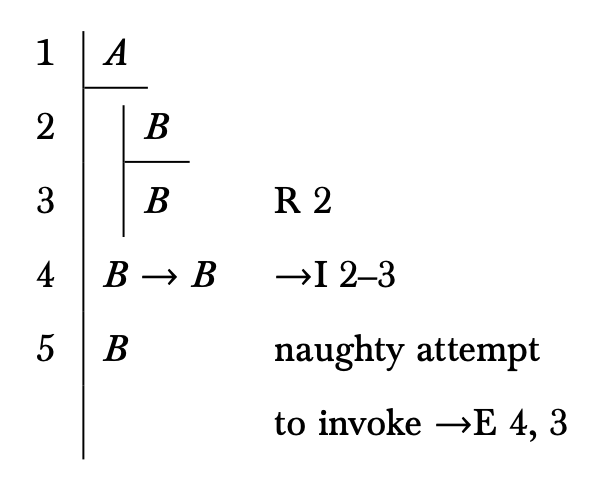
\includegraphics[width=\textwidth,height=0.65\textheight]{5_1a.png}
\caption{Bad Proof \#1 - Appeal to line inside subproof}
\end{figure}
\end{frame}

\begin{frame}{Closing One Subproof at a Time}
\protect\hypertarget{closing-one-subproof-at-a-time}{}
\begin{figure}
\centering
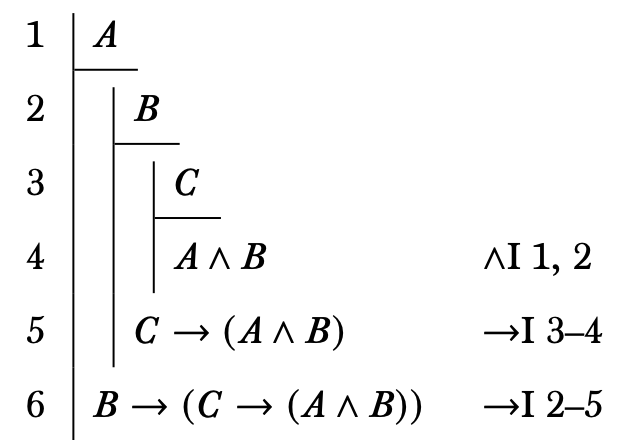
\includegraphics[width=\textwidth,height=0.65\textheight]{5_1b.png}
\caption{A good proof - closing subproofs in reverse order to opening}
\end{figure}
\end{frame}

\begin{frame}{What Could go Wrong?!}
\protect\hypertarget{what-could-go-wrong-1}{}
\begin{figure}
\centering
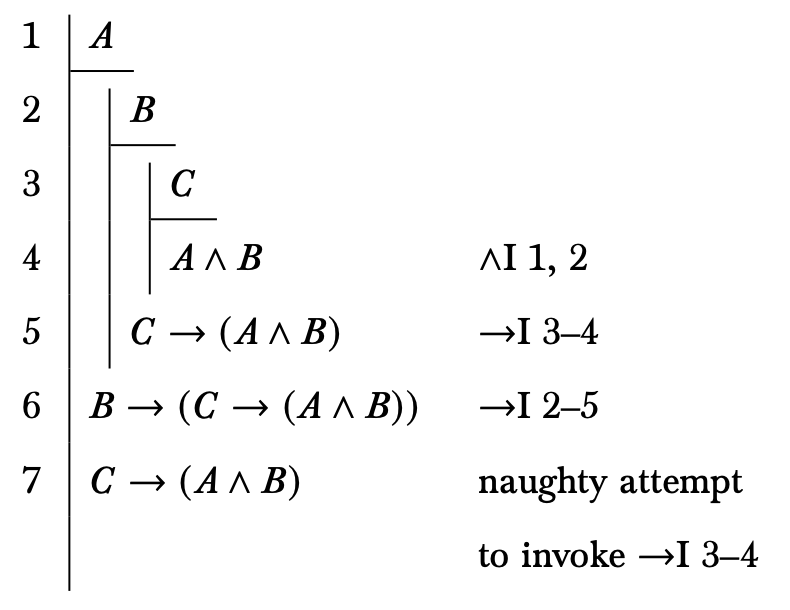
\includegraphics[width=\textwidth,height=0.65\textheight]{5_1c.png}
\caption{Bad Proof \#2 - Appeal to line inside subproof}
\end{figure}
\end{frame}

\begin{frame}{What Could go Wrong?!}
\protect\hypertarget{what-could-go-wrong-2}{}
\begin{figure}
\centering
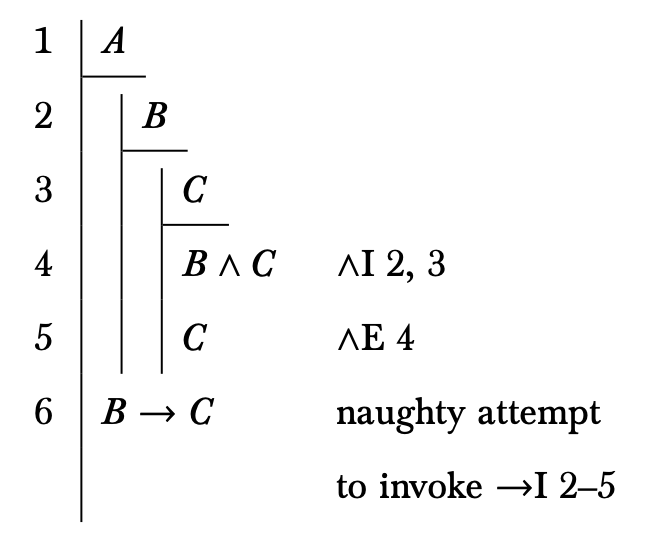
\includegraphics[width=\textwidth,height=0.65\textheight]{5_1d.png}
\caption{Bad Proof \#3 - Closing Two Subproofs at a Time}
\end{figure}
\end{frame}

\begin{frame}{Remember}
\protect\hypertarget{remember}{}
\begin{itemize}
\tightlist
\item
  Once a subproof is closed, you can only appeal to the subproof, not to
  the lines in it.
\item
  Close subproofs in reverse order to when you open them.
\item
  In any case you'll be doing, just close one at a time.
\end{itemize}
\end{frame}

\begin{frame}{For Next Time}
\protect\hypertarget{for-next-time}{}
We will look at the rules for or.
\end{frame}

\end{document}
